\chapter{Background}

Based on the high-level goals for the project, it is important to introduce the string-matching algorithms that are essential for implementation within the product. This section will explore existing visualization solutions to determine how specific features have been implemented and what improvements can be made. The idea behind this is that non-functional prototypes will be developed that can be utilised in the requirement-gathering workshop.

\section{Principal String Matching Algorithms}
\label{bac:algorithms}

As mentioned, string-matching algorithms have the role of finding a specific sequence of symbols within a larger text. There exist several algorithms that have been developed over the years, each having its advantages and drawbacks. This section introduces three such algorithms: naive approach, Knuth-Morris-Pratt (KMP), and Boyer-Moore (BM), as per the initial requirements, see Section~\ref{intro:initial_requirements}.


\subsection{Brute Force Approach}
\label{bac:brute-force}

The brute force algorithm, also known as the naive approach, involves checking each pair of characters between the text and pattern until the solution is found. The pseudocode for such an algorithm is presented in Algorithm~\ref{alg:brute_force}.

\begin{algorithm}[t]
    \DontPrintSemicolon
    \KwData{$text$ // the text we are searching}
    \KwData{$pattern$ // the pattern we are searching for}

    \Begin{
      $\mathit{textLength} \longleftarrow $ length of text\;
      $\mathit{patternLength} \longleftarrow $ length of pattern\;
      $\mathit{startingPoint} \longleftarrow 0$\;
      $\mathit{patternIndex} \longleftarrow 0$\;
      $\mathit{textIndex} \longleftarrow 0$\;

      \While{$\mathit{startingPoint} \leq (\mathit{textLength} - \mathit{patternLength}) \;\; \&\& \; \; \mathit{patternIndex} < \mathit{patternLength}$}
      {
        \If{$\mathit{text}[\mathit{textIndex}] == \mathit{pattern}[\mathit{patternIndex}]$}
        {
           $\mathit{textIndex} \longleftarrow \mathit{textIndex} + 1$\;
           $\mathit{patternIndex} \longleftarrow \mathit{patternIndex} + 1$\;
        }
        \Else{
            $\mathit{patternIndex} \longleftarrow 0$\\
            $\mathit{startingPoint} \longleftarrow \mathit{startingPoint} + 1$ \\
            $\mathit{textIndex} \longleftarrow \mathit{startingPoint}$
        }
      }

    \If{$\mathit{patternIndex} == \mathit{patternLength}$} {
        return $\mathit{startingPoint}$
    }
    return $-1$

    }
\caption{Brute Force Algorithm}
\label{alg:brute_force}
\end{algorithm}

Starting from the $\mathit{startingPoint}$ of the text, we check each pair of text characters and pattern characters one by one (this happens by incrementing the $\mathit{textIndex}$ and $\mathit{patternIndex}$ upon a match, as shown by lines 9 and 10 respectively). If any pair of characters between the text and the pattern are not equal, we move one character forward in the text (completed by lines 14 and 15) and start checking from there against the start of the pattern (since we reset the $\mathit{patternIndex}$ to be 0, as of line 13).

Assuming a text of "string" and pattern of "sting" we can show the concept visually in Figure~\ref{alg:brute_force_exec}. In this example, our $startingPoint$ is 0, as we start comparing from the first character of the text. We then managed to match "st" between the text and the pattern, moving on to the comparison between "r" and "i" at the second index of both text and pattern. Here the characters don't match, so we increase our $staringPoint$ to start comparing text from index 1 to the pattern, in our example, we now start comparing from "t" in the text and the beginning of the pattern. Such process of moving one character forward in the text, upon each mismatch repeats until the text is exhausted (i.e. the $startingPoint$ is greater than the last index that could contain the pattern, as shown in line 7) or the pattern is fully matched (the $patternIndex$ is equal to $patternLength$, also on line 7).

\begin{figure}[t]
    \centering
    \begin{tikzpicture}
        [every node/.style={anchor=base, font=\huge},
        smallnum/.style={font=\small},
        textsize/.style={font=\small}]

        \begin{scope}
            \matrix (m) [matrix of nodes, nodes in empty cells]
            {
                |[textsize]| index &
                |[smallnum]|0 & |[smallnum]|1 &  |[smallnum]|2 &  |[smallnum]|3 &
                |[smallnum]|4 & |[smallnum]|5 \\
                |[textsize]| text & |[text=green]| s & |[text=green]| t &  |[text=red]| r &  i &
                n &  g \\
                |[textsize]| pattern & |[text=green]| s & |[text=green]| t &  |[text=red]| i & n &  g \\
            };
        \end{scope}

        \begin{scope}[yshift=-3cm]
            \matrix (m1) [matrix of nodes, nodes in empty cells]
            {
                |[textsize]| index &
                |[smallnum]|0 & |[smallnum]|1 &  |[smallnum]|2 &  |[smallnum]|3 &
                |[smallnum]|4 & |[smallnum]|5 \\
                |[textsize]| text &
                s & |[text=orange]| t &  r &  i &
                n & g \\
                |[textsize]| text & & |[text=orange]|s &  t & i & n &
                g \\
            };
        \end{scope}

        \draw[->,thick] (m.south) -- (m1.north);
    \end{tikzpicture}
    \caption{Example execution of the brute force algorithm.}
    \label{alg:brute_force_exec}
\end{figure}


The time complexity of this algorithm is $O(mn)$, assuming $n$ is the length of text and $m$ is the length of the pattern. This complexity arises from the fact that in the worst case (i.e., there is no match, but we will still need to compare the full length of the pattern when starting at each character of the text, as the mismatch always occurs on the last character of the pattern) we will need to go iterate over all characters in the text and all characters in the pattern at each $\mathit{startingPoint}$ value. The space complexity is constant ($O(1)$), as we only keep track of the $\mathit{startingPoint}$, $\mathit{patternIndex}$ and $\mathit{textIndex}$. Such an approach is trivial, \gethin{what is trivial?} however, it can form a basis for introducing the problem of searching large pieces of text efficiently and highlight the need for more sophisticated methods such as ones introduced in the following sections.


\subsection{Knuth-Morris-Pratt}

Knuth-Morris-Pratt greatly improves upon its predecessor described in Section~\ref{bac:brute-force} by achieving a linear time complexity of $O(m+n)$ in the worst case, paying for it with the increased space complexity of  $O(m)$ used to store pre-processing results. Created by Donald Knuth, Vaughan Pratt, and James H. Morris (see \cite{KMP}), it is an online algorithm published in 1977, which exploits a border table to avoid backtracking within the text, a phenomenon seen in the naive approach, as we move the $startingPoint$ value by 1, but we would have already looked further in the text to previously mismatch.  The pseudocode for the algorithm can be seen in Algorithm~\ref{alg:knuth_morris_pratt}.

\gethin{see changes I have made to brute force and do the same thing for the other algorithms}

\begin{algorithm}[H]
    \DontPrintSemicolon
    \KwData{$text$, The text we are searching. .}
    \KwData{$pattern$, The pattern we are searching for.}

    \Begin{
      $textLength \longleftarrow $ length of text\;
      $patternLength \longleftarrow $ length of pattern\;
      $patternIndex \longleftarrow 0$\;
      $textIndex \longleftarrow 0$\;

      $borderTable \longleftarrow $ createBorderTable(pattern)\;

      \While{$textIndex$ < $textIndex$}
      {
        \If{$text$[$textIndex$] == $pattern$[$patternIndex$]}
        {
           $textIndex \longleftarrow textIndex + 1$\;
           $patternIndex \longleftarrow patternIndex + 1$\;
           \If{$patternIndex == patternLength$} {return $textIndex - patternIndex$}
        }
        \Else{
            \If{$borderTable$[$patternIndex$] > 0}
            {
                $patternIndex$ = $borderTable$[$patterIndex$]
            }
            \Else{
                \If{$patternIndex == 0$}{
                    $textIndex \longleftarrow textIndex + 1$\;
                }
                \Else{
                    $patternIndex \longleftarrow 0$\;
                }
            }
        }
      }
      return $-1$
    }
\caption{Knuth-Morris-Pratt Algorithm}
\label{alg:knuth_morris_pratt}
\end{algorithm}


\subsubsection{Pre-Processing -- Line 6.}
The algorithm works based on having the border table tell the system which pattern character should be compared with the current text character at the next step so that we don't have to go backwards in the text. The border table is a data structure equal in length to the pattern, with each index representing a substring of the pattern up to, but excluding character at that index. For example in the string of "ababaca", the index of 4 assuming 0-indexing would consider the string of "ababa", but without the last character, as denoted by the red outline in Figure~\ref{fig:kmp-pre-process}. Each entry of the structure contains the size of the substring that is both a prefix and suffix of the substring considered. Considering our earlier example of index 4 the prefix and suffix would be ab, which has a length of 2, as the first two characters are ab and the last two characters are also ab, denoted in blue and orange respectively.

\begin{figure}[htp]
  \centering
  \begin{tikzpicture}
    [every node/.style={anchor=base, font=\huge},
     smallnum/.style={font=\small},
     textsize/.style={font=\small}]

    \matrix (m) [matrix of nodes, nodes in empty cells]
    {
      |[textsize]| index & |[text=blue]| a & |[text=blue]| b &  |[text=orange]| a & |[text=orange]| b & a & c & a \\
      |[textsize]| pattern & |[smallnum]| 0 & |[smallnum]| 1 & |[smallnum]| 2 & |[smallnum]| 3 & |[smallnum]| 4 & |[smallnum]| 5 & |[smallnum]| 6 \\
    };

    \node[fit=(m-1-2.north west) (m-2-5.south east), draw=red, inner sep=2pt] {};
  \end{tikzpicture}
  \caption{Working out border of pattern at index 4}
  \label{fig:kmp-pre-process}
\end{figure}


\gethin{add line numbers to subsubsections below?}

\subsubsection{Match.}
Upon a match, as with the brute force algorithm, we simply move one unit along within the text and the pattern, comparing the next pair of characters. This can be seen by lines 8 to 10 being the same as the naive approach match case.

\subsubsection{Mismatch.}
There are possible 3 cases for KMP to consider when we fail to match a pair of symbols. The cases are handled in the else clause spanning lines 15 to 27, a large chunk of the entire pseudocode. The case is determined based on the border table. More specifically we index the border table using the current index of the pattern we mismatched on - the $patternIndex$. If the border table reports a non-zero value, as checked by the conditional on line 16, it means the last $x$ characters in the already matched characters, match the start of the pattern, or rather the prefix of the matched pattern so far is also the suffix. In such case, we stay on the current character of the text, but shift the pattern to match the start of it with the last $x$ characters matched in the text/pattern. Visually this can be seen below, in Figure~\ref{kmp:mismatch-case-1}


\begin{figure}[hpt]
  \centering
  \begin{tikzpicture}
    [every node/.style={anchor=base, font=\huge},
     smallnum/.style={font=\small},
     textsize/.style={font=\small}]

    \begin{scope}
      \matrix (m1) [matrix of nodes, nodes in empty cells]
      {
        |[textsize]| index &
        |[smallnum]|0 & |[smallnum]|1 &  |[smallnum]|2 &  |[smallnum]|3 &
        |[smallnum]|4 & |[smallnum]|5 & |[smallnum]| 6 \\
        |[textsize]| text & |[text=green]| a & |[text=green]| b &  |[text=green]| a & |[text=green]| b &
        |[text=green]| a &
        |[text=red]|c & a \\
      |[textsize]| pattern & |[text=green]| a & |[text=green]| b &  |[text=green]| a & |[text=green]| b &
        |[text=green]| a &
        |[text=red]|b & a \\
      };

    \end{scope}

    \begin{scope} [yshift=-2cm]
    \matrix (m) [matrix of nodes, nodes in empty cells]
    {
       |[textsize]| index & |[smallnum]| 0 & |[smallnum]| 1 & |[smallnum]| 2 & |[smallnum]| 3 & |[smallnum]| 4 & |[smallnum]| 5 & |[smallnum]| 6 \\
      |[textsize]| pattern & |[text=blue]| a & |[text=blue]| b &  |[text=brown]| a & |[text=orange]| b & |[text=orange]| a & c & a \\
    };

    \draw[->,thick] (m1.south) -- (m.north);
    \end{scope}

    \begin{scope}[yshift=-4.2cm]
      \matrix (m2) [matrix of nodes, nodes in empty cells]
      {
        |[textsize]| text &  a &  b &  |[text=green]| a & |[text=green]| b &
        |[text=green]| a &
        |[text=orange]|b & a \\
        |[textsize]| pattern &
         &
         &
        |[text=green]| a & |[text=green]| b &  |[text=green]| a & |[text=orange]| b &
        a & c & a \\
      };
    \end{scope}

    \draw[->,thick] (m.south) -- (m2.north);

  \end{tikzpicture}
  \caption{KMP Mismatch Case 1 -- $borderTable$[$patternIndex$] is not 0}
  \label{kmp:mismatch-case-1}
\end{figure}


In this example, we mismatched the letters "c" and "b" on the $patternIndex$ of 5. The border of the substring of the pattern in the range $0..5$ exists, it being "aba", since the string starts with "aba" and finishes with "aba". In such case we now set the $patternIndex$ to 3, shifting it right in relation to the text.  We continue checking from the "b" in both text and pattern.

In the case the $borderTable$ reports a value of 0, we need to also consider the $patternIndex$ value. Should the currently checked character in the pattern be the very first character, we essentially perform the naive approach step, moving one character forward in the text (shown by the increment on line 21). We now compare the pattern from the next character in the text: \gethin{reference figure or algorithm}


\begin{figure}[H]
    \centering
    \begin{tikzpicture}
        [every node/.style={anchor=base, font=\huge},
        smallnum/.style={font=\small},
        textsize/.style={font=\small}]

    \begin{scope}
      \matrix (m) [matrix of nodes, nodes in empty cells]
      {
        |[textsize]| index &
        |[smallnum]|0 & |[smallnum]|1 &  |[smallnum]|2 &  |[smallnum]|3 &
        |[smallnum]|4 & |[smallnum]|5  \\
        |[textsize]| text &  |[text=red]|  s &  t &  r &  i &
         n &  g \\
      |[textsize]| pattern & |[text=red]| k & t &  i & n &  g \\
      };

    \end{scope}

     \begin{scope}[yshift=-2.5cm]
      \matrix (m1) [matrix of nodes, nodes in empty cells]
      {
        |[textsize]| text &
        s & |[text=orange]| t &  r &  i &
        n & g \\
      |[textsize]| pattern && |[text=orange]| k &  t &  i & n &
        g \\
      };
    \end{scope}

    \draw[->,thick] (m.south) -- (m1.north);
    \end{tikzpicture}
    \caption{KMP Mismatch Case 2 -- both $borderTable$[$patternIndex$] and $patternIndex$ are 0 }
    \label{kmp:mismatch-case-2}
\end{figure}


Should be currently checked value in the pattern not be the first character, we simply start the comparison again from the current $textIndex$ by resetting the $patternIndex$, as shown by line 24. This is similar to the naive approach, but we don't move to the next character from the $startingPoint$, but restart the comparison with mismatched character in the text. Such case is show visually in Figure~\ref{kmp:mismatch-case-3}.


\begin{figure}[H]
    \centering
    \begin{tikzpicture}
        [every node/.style={anchor=base, font=\huge},
        smallnum/.style={font=\small},
        textsize/.style={font=\small}]

    \begin{scope}
      \matrix (m) [matrix of nodes, nodes in empty cells]
      {
        |[textsize]| index &
        |[smallnum]|0 & |[smallnum]|1 &  |[smallnum]|2 &  |[smallnum]|3 &
        |[smallnum]|4 & |[smallnum]|5  \\
        |[textsize]| text & |[text=green]| s & |[text=green]| t &  |[text=red]| r &  i &
         n &  g \\
      |[textsize]| pattern & |[text=green]| s & |[text=green]| t &  |[text=red]| i & n &  g \\
      };

    \end{scope}

     \begin{scope}[yshift=-3cm]
      \matrix (m1) [matrix of nodes, nodes in empty cells]
      {
        |[textsize]| text &
         s & t &  |[text=orange]| r &  i &
        n & g \\
      |[textsize]| pattern & & & |[text=orange]| s &  t &  i & n &
        g \\
      };
    \end{scope}

    \draw[->,thick] (m.south) -- (m1.north);
    \end{tikzpicture}
    \caption{KMP Mismatch Case 3 -- $borderTable$[$patternIndex$] is 0, but $patternIndex$ is not}
    \label{kmp:mismatch-case-3}
\end{figure}

Above is the same example as in Figure \ref{alg:brute_force_exec}, however this time instead of starting checking from index 1 in the text, we start checking from index 2, as there is no border - we avoid going back to index 1 in the text, as we have already been there previously and know it cannot match "r" there.


\subsection{Boyer-Moore Algorithm Horsepool}

Boyer-Moore is an algorithm introduced in 1975, as summarised by \cite{bm}, before the dawn of KMP. On paper it appears slower than its ancestor, as its worst time complexity is $O(nm)$, however, it has been found that its performance is almost always better in practice. The reason for such a phenomenon is the fact BM is prone to skipping many characters per step, quickly eliminating areas of the text that cannot possibly match the pattern. Recently \cite{KMPvsBM} showed that BM outperformed KMP almost every single time, in some cases reaching one-third of the time it takes KMP to run.

Similar to KMP, the algorithm utilises a pre-processing data structure, which determines the next comparison during execution. Unlike the 2 previous algorithms, it works based on comparing right to left, starting the comparison from the last character in the pattern to the corresponding character in the text. There exist many variations, however, for this project, the focus was the Horsepool variant, a version using the "bad-character" rule only, as opposed to both the "bad-character" and "good-suffix" rules. It is important to note that the horsepool variant is more commonly used as the original algorithm provides little to no performance benefits \cite{horsepool_vs_full}, specifically due to little impact from the good-suffix rule. The pseudocode for the variant is as follows:


\begin{algorithm}[H]
    \DontPrintSemicolon
    \KwData{$text$, The text we are searching. .}
    \KwData{$pattern$, The pattern we are searching for.}

    \Begin{
      $textLength \longleftarrow $ length of text\;
      $patternLength \longleftarrow $ length of pattern\;
      $startingPoint \longleftarrow 0$\;
      $patternIndex \longleftarrow patternLength - 1$\;
      $textIndex \longleftarrow patternLength - 1$\;

      $lastOccurrenceTable \longleftarrow $ createLastOccurrenceTable(pattern)\;

      \While{$startingPoint$ <= ($textLength$ - $patternLength$) $\&\&$ $patternIndex$ >= $0$}
      {
        \If{$text$[$textIndex$] == $pattern$[$patternIndex$]}
        {
           $textIndex \longleftarrow textIndex - 1$\;
           $patternIndex \longleftarrow patternIndex - 1$\;
           \If{$patternIndex == patternLength$} {return $textIndex - patternIndex$}
        }
        \Else{
            $startingPoint \longleftarrow startingPoint + max(1, patternIndex  - lastOccurrenceTable[text[textIndex]])$\;
            $textIndex \longleftarrow textLength - min(patternIndex, 1  + lastOccurrenceTable[text[textIndex]])$\;
            $patternIndex \longleftarrow pattenLength - 1$\;
        }
      }
      \If{$patternIndex$ < $0$} {
        return $startingPoint$
      }
      return $-1$
    }
\caption{Boyer-Moore Algorithm}
\label{alg:boyer_moore}
\end{algorithm}


\subsubsection{Pre-Processing and The Bad Character Rule} On line 7, the execution context is changed to a function that creates a dictionary of the last occurrence. As mentioned this is a data structure, which supports the algorithm during execution by storing the last index of each character in the pattern. For example in the word "ababa", the last occurrence would look as follows:
\begin{itemize}
    \item{a : 4}
    \item{b : 3}
\end{itemize}


\subsubsection{Match} Upon a match, lines 10 and 11 show $textIndex$ and $patternIndex$ are both decreased. This is due to the fact we check right to left, instead of left to right, meaning characters to the right are already matched.

\subsubsection{Mismatch} Upon a mismatch, there are 3 possible things that can happen during execution.  In the first case the last occurrence of mismatched character in text has not been matched yet i.e. the last occurrence exists to the left of currently checked pattern character. In such situation, we need to shift the pattern in such way to line up the last occurrence with the current text element we are looking at.  Referring to example in Figure~\ref{bm:mismatch-case-1}, we need the "a" in the pattern to be moved to the right until lined up with the mismatched a in the test.

\begin{figure}[H]
  \centering
  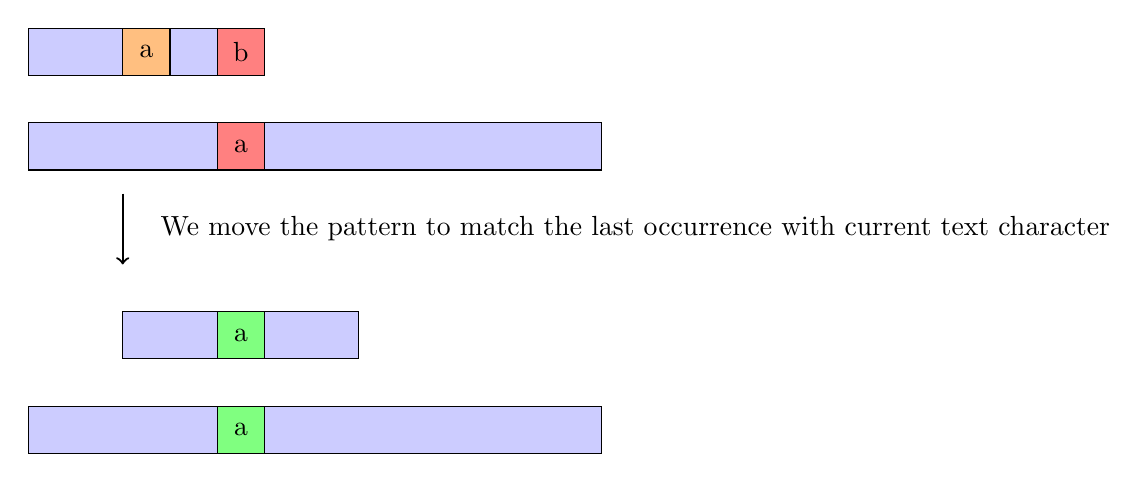
\begin{tikzpicture}[scale=0.6]
    \begin{scope}
        \draw [draw=black, fill=blue!20] (0,0) rectangle (4,1);
        \draw [draw=black, fill=red!50] (4, 0) rectangle (5, 1) node[midway] {b};;
        \draw [draw=black, fill=orange!50] (2,0) rectangle (3,1) node[midway] {a};
        \draw [draw=black, fill=blue!20] (0, -2) rectangle (\textwidth, -1);
        \draw [draw=black, fill=red!50] (4, -2) rectangle (5, -1) node[midway] {a};;
    \end{scope}

    \draw[->, thick] (2, -2.5) -- (2, -4)  node[midway, right, xshift=10pt] {We move the pattern to match the last occurrence with current text character};

    \begin{scope}
        \draw [draw=black, fill=blue!20] (2,-6) rectangle (7,-5);
        \draw [draw=black, fill=green!50] (4,-6) rectangle (5,-5) node[midway] {a};;
        \draw [draw=black, fill=blue!20] (0, -8) rectangle (\textwidth, -7);
        \draw [draw=black, fill=green!50] (4, -8) rectangle (5, -7) node[midway] {a};;
    \end{scope}
  \end{tikzpicture}
  \caption{Boyer-Moore Mismatch Case 1}
  \label{bm:mismatch-case-1}
\end{figure}


With case 2, the last occurrence of the mismatched character has already been matched i.e the last occurrence is to the right of currently checked pattern character. In such case we simply move the pattern one place forward respective to the text (increment the $textIndex$ by 1 )and restart the search from the end of the string. This happens because we cannot guarantee no match, since there could be another instance of the character within the pattern to match the text, one that is not the last occurrence. Figure \ref{bm:mismatch-case-2} shows such case.

\begin{figure}[H]
  \centering
  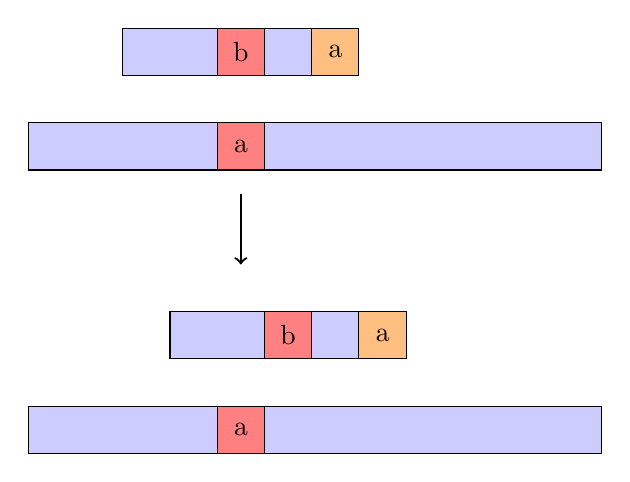
\begin{tikzpicture}[scale=0.6]
    \begin{scope}
        \draw [draw=black, fill=blue!20] (2,0) rectangle (7,1);
        \draw [draw=black, fill=red!50] (4, 0) rectangle (5, 1) node[midway] {b};;
        \draw [draw=black, fill=orange!50] (6,0) rectangle (7,1) node[midway] {a};
        \draw [draw=black, fill=blue!20] (0, -2) rectangle (\textwidth, -1);
        \draw [draw=black, fill=red!50] (4, -2) rectangle (5, -1) node[midway] {a};;
    \end{scope}

    \draw[->, thick] (4.5, -2.5) -- (4.5, -4); % Centering the arrow horizontally

    \begin{scope}
        \draw [draw=black, fill=blue!20] (3,-6) rectangle (8,-5);
        \draw [draw=black, fill=red!50] (5,-6) rectangle (6,-5) node[midway] {b};;
        \draw [draw=black, fill=orange!50] (7,-6) rectangle (8,-5) node[midway] {a};
        \draw [draw=black, fill=blue!20] (0, -8) rectangle (\textwidth, -7);
        \draw [draw=black, fill=red!50] (4, -8) rectangle (5, -7) node[midway] {a};;
    \end{scope}

  \end{tikzpicture}
  \caption{Boyer-Moore Mismatch Case 2}
  \label{bm:mismatch-case-2}
\end{figure}


The final case covers the situation where there is  no last occurrence for a text character, simply the character does not appear in the pattern. In such case we we move the pattern past the mismatched element i.e. we start checking the text from the next element, as it is impossible to match any substring where the pattern character does not exist. Visually this can be seen as:

\begin{figure}[H]
  \centering
  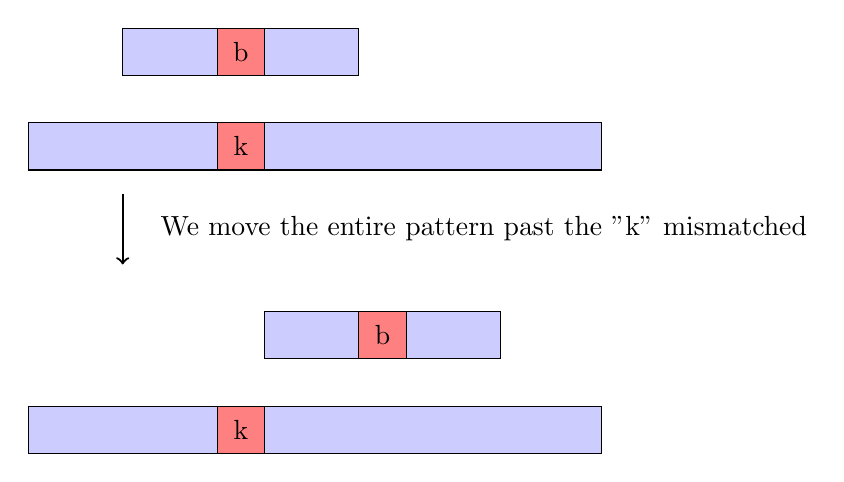
\begin{tikzpicture}[scale=0.6]
    \begin{scope}
        \draw [draw=black, fill=blue!20] (2,0) rectangle (7,1);
        \draw [draw=black, fill=red!50] (4, 0) rectangle (5, 1) node[midway] {b};;
        \draw [draw=black, fill=blue!20] (0, -2) rectangle (\textwidth, -1);
        \draw [draw=black, fill=red!50] (4, -2) rectangle (5, -1) node[midway] {k};;
    \end{scope}

    \draw[->, thick] (2, -2.5) -- (2, -4)  node[midway, right, xshift=10pt] {We move the entire pattern past the "k" mismatched};


    \begin{scope}
        \draw [draw=black, fill=blue!20] (5,-6) rectangle (10,-5);
        \draw [draw=black, fill=red!50] (7,-6) rectangle (8,-5) node[midway] {b};;
        \draw [draw=black, fill=blue!20] (0, -8) rectangle (\textwidth, -7);
        \draw [draw=black, fill=red!50] (4, -8) rectangle (5, -7) node[midway] {k};;
    \end{scope}

  \end{tikzpicture}
  \caption{Boyer-Moore Mismatch Case 3}
  \label{bm:mismatch-case-3}
\end{figure}


The 3 cases combined make up the algorithm, over the years the 3 cases have been optimised to 3 variable equations defined between lines 17-19, which won't be explained here, but for more information, refer to this resource \cite{}.


\section{Existing Products}
\label{bac:existing_products}

There exists a plethora of software applications made and published to educate in regards to  string-matching algorithms. Each solution takes a different approach to the design of the software application. Some focus more on creating a visually appealing and user-friendly interface, while others prioritize the functionality and features of the application. Ultimately, the approach taken depends on the target audience's needs and experiences as well as the goals of the project. This section will summarise the solutions explored, discuss the advantages and disadvantages of each and concluding with the details that will be use within the prototypes of the requirement-gathering workshop. The features chosen can be seen in wireframes 1 through to 3 in Appendix~\ref{app:initial_wireframes}.

\subsection{\href{https://cmps-people.ok.ubc.ca/ylucet/DS/Algorithms.html}{Data Structure Visualizations}}

The original Java-based version of this application was developed by David Galles of the University of San Francisco in 2011, however the current website Flash-based version is an updated application developed by Yves Lucet of I. K. Barber School of Arts \& Sciences, UBC Okanagan. The application contains visualisers for algorithms from a range of areas, not only string-matching, including, for example, Heap-related algorithms. The range of applcaitions makes the application useful for any Computer Science student, teacher, professional or enthusiast.  Being ranked quite highly on the search engine results suggests it is also a very popular visualiser enjoyed by many people --making it a defacto product for analyse.

Advantages of this applcation:
\begin{itemize}
    \item \textbf{Custom text and pattern.} It is possible to execute the algorithms with custom text and pattern, making it possible to adapt the execution to the user's case.
    \item \textbf{"Failure function" building for KMP.}  The visualiser shows how the preprocessing steps for KMP are completed, albeit a different method to the one in Algorithmics \Romannum{1}.
    \item \textbf{Reset.} The site can reset everything to default values, always giving the user an out when something is going wrong - in line with usability heuristic number 3, created by \cite{Nielsen_2024}, by giving users an "emergency exit".
    \item \textbf{Stepping forward and backward.} The user can step forward and backwards one step at a time.
    \item \textbf{Skipping to first and last step.} The user can go all the way to the start or the end should they wish.
    \item \textbf{Pause/Play.} The user can pause execution and later resume it.
    \item \textbf{Animation Speed.} It is possible to change how quickly the animation goes through the steps.
    \item \textbf{Canvas size change.}  The site gives the ability to set the canvas size to exact measurements wished by the user.
    \item \textbf{Change control location.} A quality-of-life feature, where the user can place the control dashboard either as a header or a footer.
    \item \textbf{Addition of new algorithm.} There is a guide, which can be followed to add a new algorithm to visualise.
\end{itemize}


Disadvantages of the application:
\begin{itemize}
    \item \textbf{Cannot reset while running.} The visualizer controls are not very intuitive. You can only reset at the final step, and using the skip functionality sometimes crashes the site.
    \item \textbf{Out-of-date aesthetics.} The website looks quite dated, which may put off some users from using it and instead looking for an alternative.
    \item \textbf{Difficult to follow tutorial.} The tutorial is quite involved and requires some understanding of the massive codebase. While possible, it is not easy to add a new algorithm.
    \item \textbf{Difficult to read certain elements.} The animation is never resized, hence some elements can be difficult to read, especially on larger displays.
    \item \textbf{Not mobile-friendly.} Although the animation is fairly visible, a horizontal scroll is required to access all control elements on a smaller screen.
    \item \textbf{Lacking the Brute Force Algorithm.} No animations for the naive approach are implemented at all.
\end{itemize}


% \begin{longtable}{|p{0.45\linewidth}|p{0.45\linewidth}|}
% \hline
% \textbf{Advantages} & \textbf{Disadvantages} \\ \hline
% \endhead
% \begin{itemize}[leftmargin=*]
%     \item \textbf{Custom text and pattern}: It is possible to execute the algorithms with custom text and pattern.
%     \item \textbf{"Failure function" building for KMP}: The visualiser shows how the preprocessing steps for KMP are completed, albeit a different method to the one in Algorithmics \Romannum{1}.
%     \item \textbf{Reset}: The site has the ability to reset everything to default values, always giving the user an out when something is going wrong.
%     \item \textbf{Stepping forward and backward}: The user is able to step forward and backward one step at a time.
%     \item \textbf{Skipping to first and last step}: The user is able to go all the way to the start or the end should they wish.
%     \item \textbf{Pause/Play}: The user is able to pause execution and later resume it.
%     \item \textbf{Animation Speed}: It is possible to change how quickly the animation goes through the steps.
%     \item \textbf{Canvas size change}: The site gives the ability to set the canvas size to exact measurements wished by the user.
%     \item \textbf{Change control location}: A quality of life feature, where the user can place the control dashboard either as a header or a footer.
%     \item \textbf{Addition of new algorithm}: There is a guide, which can be followed to add a new algorithm to visualize.
% \end{itemize} &
% \begin{itemize}[leftmargin=*]
%     \item \textbf{Cannot reset while running}: The controls are quite clunky when the visualiser is running. It is only possible to reset when reaching the final step. I also found sometimes using the skip functionality breaks the entire site, forcing the user to reload.
%     \item \textbf{Out-of-date aesthetics}: The website looks quite dated, which may put off some users from using it and instead looking for an alternative.
%     \item \textbf{Difficult to follow tutorial for extension}: The tutorial is quite involved and requires some understanding of the massive codebase.
%     \item \textbf{Difficult to read certain elements}: The animation is never resized, hence some elements can be difficult to read, especially on larger displays.
%     \item \textbf{No mobile-friendly}: Although the animation is fairly visible, a horizontal scroll is required to access all control elements.
% \end{itemize} \\ \hline
% \end{longtable}

Overall the product does a great job at educating via great animations for a wide range of algorithms, also providing a vast spectrum of quality-of-life features, attempting to make the learning process as frictionless for the user as possible. However the product is also quite dated and several features of the app are not functioning smoothly, some appearing to be causing crashes on the site. The UI experience is hence not optimal, likely causing the user to look for an alternative learning tool. For my wireframes, I decided to implement a version of the animation style (the use of squares and highlighting of their border), as well as the pause/play, go forward, go backwards and the animation speed setter features, as I thought all of these made it easier to understand the KMP and BM algorithms.

\subsection{\href{https://algorithm-visualizer.org/}{Algorithm Visualizer}}

Another website that holds a large selection of algorithms and concepts to visualise, however, it adds a modern spin onto the UI design, as well as providing a lot of quality-of-life features to the user.   It is an open-source effort, where anyone can add a new visualisation.

Advantages of the application:
\begin{itemize}
    \item \textbf{Custom text and pattern.} It is possible to execute the algorithms with custom text and pattern.
    \item \textbf{Border table building for KMP.}  The visualiser shows how the preprocessing steps for KMP are completed, utilising the same concepts as in Algorithmics \Romannum{1}.
    \item \textbf{Reset.} The site can reset everything to default values, always giving the user an out when something is going wrong.
    \item \textbf{Stepping forward and backward.} The user can step forward and backwards one step at a time.
    \item \textbf{Setting exact step.} The platform provides a range element, which can be toggled to any step in the execution.
    \item \textbf{Pause/Play.} The user can pause execution and later resume it.
    \item \textbf{Animation Speed.} It is possible to change how quickly the animation goes through the steps.
    \item \textbf{Animation size change.}  The scroll-wheel of the mouse can be used to zoom into the animation, should anything not be visible.
    \item \textbf{Seperate and resizeable canvases.} Separate UI elements are used to show preprocessing steps and the actual algorithm execution - making it easy to tell what is doing what. On top of this, each is resizeable, allowing users to place focus on whatever part they struggle to understand.
    \item \textbf{Addition of new algorithms.} There is a guide and custom library, which can be utilised to add a new algorithm. This can even be done on the online platform itself - acting as an online code editor.
    \item \textbf{Source code on Github.} The source code is located on Github so that it can be easily forked or modified by anyone to meet their wishes.
    \item \textbf{Algorithm Description} Contains basic information about the algorithm in a README file, as well as the complexity.
    \item \textbf{Psuedocode Highlighting.} The animation is accompanied by the pseudocode, which is highlighted according to the step currently on.
    \item \textbf{Full screen} The UI allows the user to go full screen with the animation, on top of being able to hide the pseudocode if required.
    \item \textbf{Sign-In.} The site has a sign-in feature integration via Github, allowing changes to be made on your account e.g. visualisation of a new algorithm.
\end{itemize}


Disadvantages of the application:
\begin{itemize}
    \item \textbf{Unclear execution.} I have noticed that the animations on the website are difficult to comprehend. The pattern is not displayed clearly concerning the text being searched, and there are no descriptive messages to explain the current execution state.
    \item \textbf{No BM or the naive approach implemented.} The site only implements the KMP algorithm, lacking an animation for other principal string matching algorithms.
    \item \textbf{Pseudocode contains library calls.} The pseudocode includes visualization statements to the custom drawing library (tracers.js), which can make the code more difficult to understand, especially given its inherent complexity as Javascript code as opposed to pseudocode.
    \item \textbf{Not mobile-friendly.} The app can be seen well on a small screen, however there is no focus on the animation, making this specific element hard to see.
    \item \textbf{Controls for README.} The site contains a README to display information regarding the algorithm, however when displayed, the controls are still enabled, which makes the UI quite confusing, as the user might find it hard to work out what will happen if play is pressed.
\end{itemize}


The algorithm-visualizer.org platform does a great job at creating a medium, where it is easy to add a new visualisation for everyone to see. The custom library seems to be quite easy to understand, with comprehensive documentation being found on GitHub. However, I believe the visualization for KMP and some other unrelated ones is confusing and simply difficult to understand. On a more positive note, the code highlight feature is a great tool for visual learners, which helps users understand how each step of the animation relates to the actual code for the algorithm. This makes it easier for users to follow along and comprehend the logic behind the algorithm. I have decided to add such a feature to the first wireframe, however, remove any library-related statements, focusing only on the algorithm in question.


\subsection{\href{https://lobb.nz/stringmatchvisualiser/stringmatching.html}{String matching algorithm visualiser}}

This is a resource that contains all the principal algorithms for this project. It is also a website, however it is much simpler than the previous two solution analysed that contains all the necessary features to constitute effective learning for the user.

Advantages:
\begin{itemize}
    \item \textbf{Custom text and pattern.} It is possible to execute the algorithms with custom text and pattern.
    \item \textbf{Stepping forward and backward.} The user can step forward and backwards one step at a time.
    \item \textbf{Setting exact step.} The platform provides a range element, which can be toggled to any step in the execution.
    \item \textbf{Algorithm Description.} Contains basic information about the algorithm in a README file, which can be toggled on and off, depending on preference.
    \item \textbf{Variable Values.} Contains the current variable value held by the algorithm during execution.
    \item \textbf{Code Export.} Allows the user to export the Javascript code for the algorithm as a raw text file. It means the user can use the code to use in their project or adapt it to their needs.
    \item \textbf{Comparison Trajectory.} There exists a graph that at a glance shows where the matches, mismatches and full matches occur, allowing for setting the exact step of interest.
    \item \textbf{Simple, Clear UI.} The UI here is quite minimalistic, limiting distractions for the user and maximising the learning process.
    \item \textbf{Full Boyer-Moore.} The algorithm implements the Full Boyer-Moore version, an extension of the BM version, which will be implemented in this product.
\end{itemize}


Disadvantages:
\begin{itemize}
    \item \textbf{No play/pause functionality.}
    \item \textbf{No preprocessing visualisations.} The preprocessing elements simply exist from the start, the user cannot get an intuition behind their generation.
    \item \textbf{Not always clear what is happening.} There is no pseudocode visible on the site or a message explaining what is happening, which sometimes makes it easy to get confused about what the algorithm did.
    \item \textbf{Not mobile-friendly.} The animation and comparison trajectory both get cut off on a smaller screen, although other elements do a great job of being flexible.
\end{itemize}

The website is great at making it easy to learn about the algorithms, even making it easy to learn about the Full Boyer-Moore algorithm, which is quite challenging to implement and learn about. The pseudocode export feature and variable values display were extracted for my prototypes.


% \lstinputlisting[label = {lst:bm}, caption=Boyer-Moore Pseudocode, frame=single, columns=fullflexible]{code/boyer-moore.txt}

% \begin{figure}[H]
%   \centering
%   \begin{tikzpicture}
%     \begin{scope}
%         \draw [draw=black, fill=blue!20] (0,0) rectangle (4,1);
%         \draw [draw=black, fill=red!50] (4, 0) rectangle (5, 1) node[midway] {b};;
%         \draw [draw=black, fill=orange!50] (2,0) rectangle (3,1) node[midway] {a};
%         \draw [draw=black, fill=blue!20] (0, -2) rectangle (\textwidth, -1);
%         \draw [draw=black, fill=red!50] (4, -2) rectangle (5, -1) node[midway] {a};;
%     \end{scope}

%     \draw[->, thick] (2, -2.5) -- (2, -4)  node[midway, right, xshift=10pt] {We move the pattern to match the last occurrence with current text character};

%     \begin{scope}
%         \draw [draw=black, fill=blue!20] (2,-6) rectangle (7,-5);
%         \draw [draw=black, fill=green!50] (4,-6) rectangle (5,-5) node[midway] {a};;
%         \draw [draw=black, fill=blue!20] (0, -8) rectangle (\textwidth, -7);
%         \draw [draw=black, fill=green!50] (4, -8) rectangle (5, -7) node[midway] {a};;
%     \end{scope}
%   \end{tikzpicture}
%   \caption{Boyer-Moore Mismatch Case 1}
%   \label{bm:mismatch-case-1}
% \end{figure}







% BRUTE FORCE NOTES
% After setting up our initial variables, the naive approach involves going over each character in text and starting from such character, checking if each subsequent character matches the corresponding pattern character, if we assume the starting character corresponds to starting character of the pattern. This is done by incrementing the index of the text and pattern by 1 upon a match or upon a mismatch moving onto the next character of the text and resetting to the start of the pattern. If all symbols of the pattern match we can report a find, terminating the algorithm, otherwise we return something indicating failure in terms of the search. The pseudocode for this approach can be seen below, in Listing~\ref{lst:brute}.

% \lstinputlisting[label = {lst:brute}, caption=Brute Force Pseudocode, frame=single, columns=fullflexible]{code/brute-force.txt}

% The time complexity of this algorithm is $O(mn)$, assuming n is the length of text and m is the length of the pattern. Such complexity arises from the fact that in the worst case (i.e. no match, but we will still need to compare the full length of pattern at each character of text , as the mismatch always occurs on the last character of pattern) we will need to go iterate over all characters in the text and all characters in the pattern at each iteration. The space complexity is constant ($O(1)$), as we only keep track of the $patternIndex$ and $textIndex$.
% \\
% \\
% Such approach is trivial, however it can form a basis for introducing the problem of searching large pieces of text efficiently and highlight the need of more sophisticated methods such as ones introduced in the following sections.



% KNUTH MORRIS PRATT NOTES
% Contrasting when the border table reports a non-zero value, it means the last $x$ characters in the already matched characters, match the start of the pattern. In such case we stay on the current character of the text, but shift the pattern to match the start of it with the aforementioned matching $x$ characters in the text. Visually this can be seen in Figure~\ref{kmp:mismatch-case-2}, where upon a mismatch of c and b, we work out the border of the pattern at c, which is "aba". We therefore need to move the pattern in a way where its start of aba, matches the already matched aba at the end of the text chunk we looked through so far.





% The algorithm pseudocode involving all the cases is outlined below:
% \lstinputlisting[label = {lst:kmp}, caption=Knuth-Morris-Pratt Pseudocode, frame=single, columns=fullflexible]{code/brute-force.txt}



% \begin{figure}[H]
%   \centering
%   \begin{tikzpicture}
%     \begin{scope}
%         \draw [draw=black, fill=blue!20] (0,0) rectangle (4,1);
%         \draw [draw=black, fill=red!50] (4, 0) rectangle (5, 1) node[midway] {b};;
%         \draw [draw=black, fill=orange!50] (2,0) rectangle (3,1) node[midway] {a};
%         \draw [draw=black, fill=blue!20] (0, -2) rectangle (\textwidth, -1);
%         \draw [draw=black, fill=red!50] (4, -2) rectangle (5, -1) node[midway] {a};;
%     \end{scope}

%     \draw[->, thick] (2, -2.5) -- (2, -4)  node[midway, right, xshift=10pt] {We move the pattern to match the last occurrence with current text character};

%     \begin{scope}
%         \draw [draw=black, fill=blue!20] (2,-6) rectangle (7,-5);
%         \draw [draw=black, fill=green!50] (4,-6) rectangle (5,-5) node[midway] {a};;
%         \draw [draw=black, fill=blue!20] (0, -8) rectangle (\textwidth, -7);
%         \draw [draw=black, fill=green!50] (4, -8) rectangle (5, -7) node[midway] {a};;
%     \end{scope}
%   \end{tikzpicture}
%   \caption{Boyer-Moore Mismatch Case 1}
%   \label{bm:mismatch-case-1}
% \end{figure}
